% !TEX TS-program = xelatex
% !TEX encoding = UTF-8
\documentclass[12pt,a4paper]{article}
\usepackage{graphicx}
\usepackage[UTF8, heading=true]{ctex}
\usepackage{fancyhdr}
\usepackage{indentfirst}
\usepackage{amsmath}
\graphicspath{{figures/}}
\usepackage{tikz}
%\usepackage{CJK}
\usepackage{url}
\usepackage{array}

%\setcounter{secnumdepth}{3}
%\renewcommand\thesection{\arabic {section}}
\usepackage{tabularx}
%\usepackage{float}
\usepackage{subcaption}
\usepackage{caption}
\usepackage[section]{placeins}
\usepackage{ruby}
\usepackage[backend=biber,bibstyle=gb7714-2015,%nature,%
citestyle=gb7714-2015%,backref=true%
]{biblatex}
\usepackage[unicode,colorlinks=true,pdfstartview=FitH,
linkcolor=blue,anchorcolor=violet,citecolor=magenta
]{hyperref}

\pagestyle{fancy}
%\renewcommand{\chaptermark}[1]{\markboth{#1}{}}
\renewcommand{\sectionmark}[1]{\markright{\thesection\ #1}}
\fancyhf{} % 清空当前的页眉页脚
\fancyfoot[C]{\thepage}
\fancyhead[LO]{\bfseries\rightmark}
\fancyhead[RE]{\bfseries\leftmark}
\renewcommand{\headrulewidth}{0.4pt} % 注意不用 \setlength
\renewcommand{\footrulewidth}{0pt}

\addbibresource[location=local]{cite.bib}

\begin{document}
%%%%%%%%%%%%%%%%%%%%%%%%%%%%%%
%% 封面部分
%%%%%%%%%%%%%%%%%%%%%%%%%%%%%%
\begin{titlepage}
    \centering
    
\includegraphics[width=0.2\textwidth]{sf1.png}\par
    \vspace{1cm}
    
\includegraphics[width=0.8\textwidth]{sf.jpg}\par
    \vspace{0.1cm}
    {\scshape\LARGE Harbin Institute of Technology \par}
    \vspace{1cm}
    {\kaishu\LARGE 面向微系统的图像测试技术课程报告\par}
    \vspace{1.5cm}
    {\huge\bfseries 圆孔图像提取与识别\par}
    \vspace{2cm}
    {\fangsong\Large\itshape 卢XX, 张XX\par}
    \vfill
    {**********, **********}\par
    \fangsong{自动化测试与控制系}

    \vfill
    指导教师	\textsc{金鹏}
    \vfill
% Bottom of the page
    {\large \today\par}
\end{titlepage}

\section{引~~~~言}

MEMS技术是近年来随着微电子技术的不断成熟而发展起来的一门新兴的交叉学科。 
其涵盖领域包括光学、机械、电子、计算机等诸多门类。 
随着MEMS技术发展及应用的扩展,对其微细结构的性能及结构的测试要求也日益迫切。 
由于其结构尺度属微纳米量级,因此传统意义的测试技术,几乎无能为力。 
本文针对MEMS装配领域中的目标物识别,通过图象处理处理手段,
利用计算机技术及CCD图像采集,进行微型圆孔的自动图像识别。

\section{设计要求}

\begin{figure}[!htb]
    \centering
    \subcaptionbox{A组}{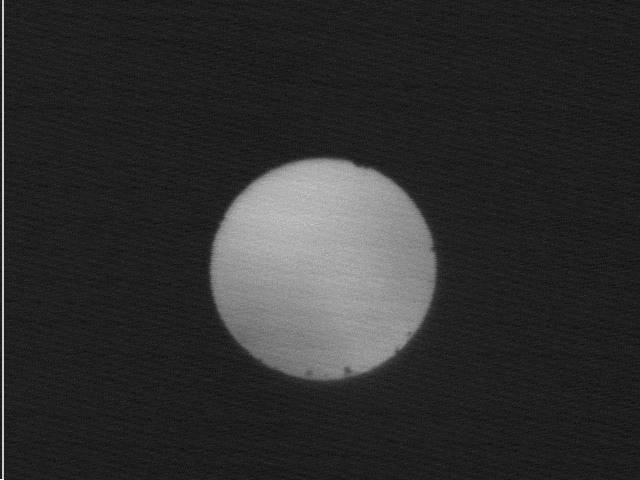
\includegraphics[width = 0.48\linewidth]{A.png}}\hfill
    \subcaptionbox{B组}{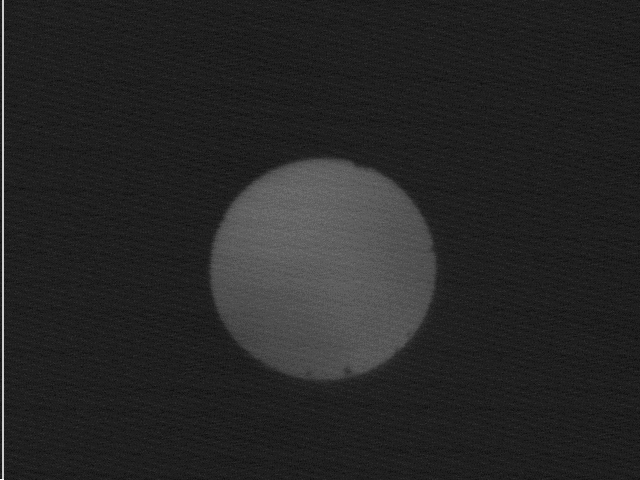
\includegraphics[width = 0.48\linewidth]{B.png}}\\
    \subcaptionbox{C组}{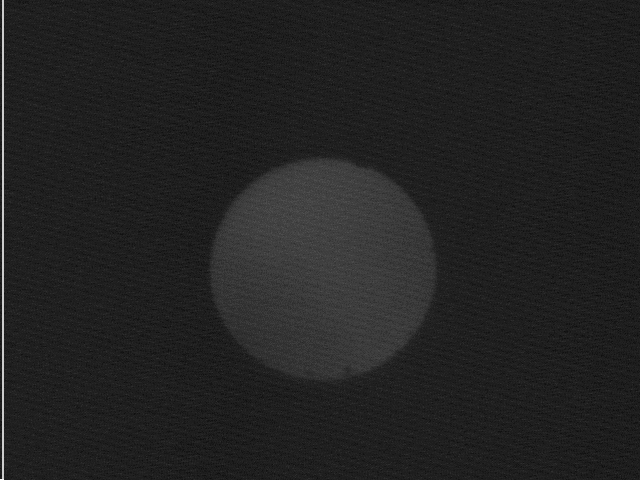
\includegraphics[width = 0.48\linewidth]{C.png}}
    \caption{采集图像}\label{fig:origin}
\end{figure}

图\ref{fig:origin} 为CCD在不同曝光时间内采集到的微型圆孔图像。
要求从图中提取出边缘信息,能够拟合出圆心和半径等参数, 
同时,要求能尽可能多的保留圆上的缺陷等细节信息,
且处理算法应具有一定的兼容性,以便日后能够实际应用。

\section{研究方法}

虽然直接按传统方法难以准确有效地识别此类图像,
但通过对传统方法的分析和组合,尝试出了一种行之有效的处理流程:
\begin{itemize}
    \item 第一步,滤波降噪;
    \item 第二步,二值化处理;
    \item 第三步,边缘检测;
    \item 第四步,提取边缘,拟合圆,计算圆心和半径。
\end{itemize}

这四步基本每一步所用的都是传统算法,通过合理的排列使之得以有效的识别。

\subsection{滤波算法}

根据设计要求,滤波算法的选取应该既能够降低噪声,又可以保持图形的边缘形态。
由于能力限制,最终在程序中提供的滤波算法只有四种:
\begin{description}
    \item[均值滤波] 线性滤波,边缘保持能力差。
    \item[高斯滤波] 线性滤波,边缘保持能力较差。
    \item[中值滤波] 非线性滤波,边缘保持能力较好。
    \item[均值平移滤波] 非线性滤波,边缘保持能力好,但性能较差。
\end{description}
这其中,均值滤波基本就是拿来练手的,基本没有实用意义。

线性滤波基于卷积\cite{KernelWiki}实现。
均值滤波使用权值相等的卷积核;
而高斯滤波的所用卷积核按高斯分布分配权值。

\begin{figure}[!htb]
    \centering
    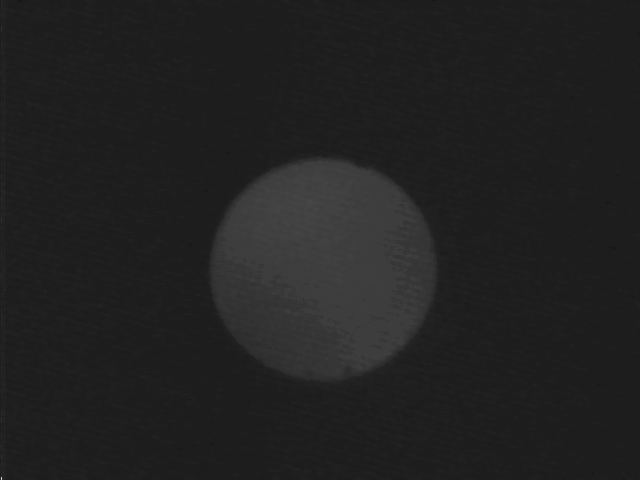
\includegraphics[width = 0.6\linewidth]{median.png}
    \caption{中值滤波}\label{fig:median}
\end{figure}

中值滤波将每个像素用其周围像素的中位数替代。
它不引入新的像素值,故具有一定的边缘保持能力。
同时,它也是这几种方法中唯一能滤除图像左侧边缘的白线的方法,
如图\ref{fig:median}所示。

\begin{figure}[!htb]
    \centering
    \subcaptionbox{A组滤波结果}{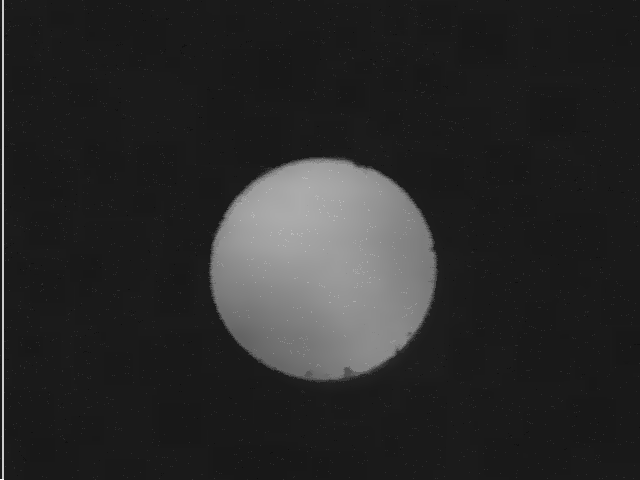
\includegraphics[width = 0.48\linewidth]{A-meanshift.png}}\hfill
    \subcaptionbox{C组滤波结果}{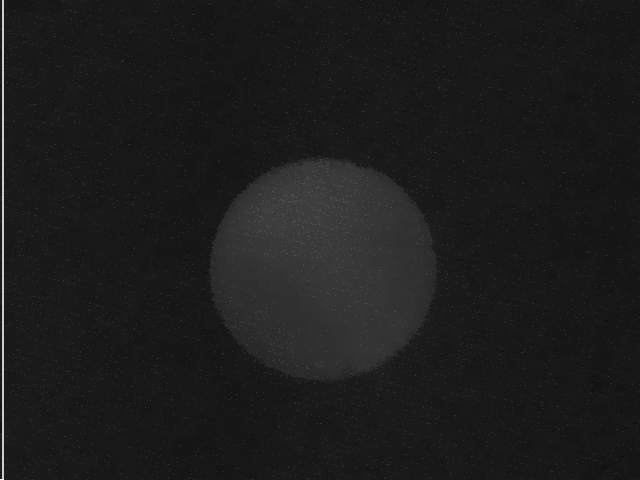
\includegraphics[width = 0.48\linewidth]{C-meanshift.png}}
    \caption{均值平移滤波}\label{fig:meanshift}
\end{figure}

均值平移滤波\cite{MeanShiftWiki}同时考虑了空间距离和灰度距离,
只有同时在像素的空间邻域和灰度邻域内才计入平均值计算。
在边缘处,像素的灰度变化通常较大,
选取合适的灰度邻域范围,边缘另一侧的像素可以不被计入平均值计算,
因而具有一定的边缘保持能力。
但当图像曝光较差时,噪声的灰度可能和图形本身的灰度相当。
此时若要继续保持边缘,则难以有效降噪。
如图\ref{fig:meanshift}所示。

\subsection{二值化之阈值分割算法}

二值化本身的算法并没有什么特别的,就是普通的单一阈值分割。
重要的是选取阈值所用的方法。

程序中尝试了以下方法:
\begin{itemize}
    \item 灰度平均值法
    \item P-Tile比例阈值法
    \item 力矩保持法\cite{Tsai1985Moment}
    \item 大津法\cite{Otsu1979A}
    \item 模糊度阈值分割法\cite{Huang1995Image}
\end{itemize}

\begin{figure}[!htbp]
    \centering
    \begin{minipage}{0.48\linewidth}
        \centering
        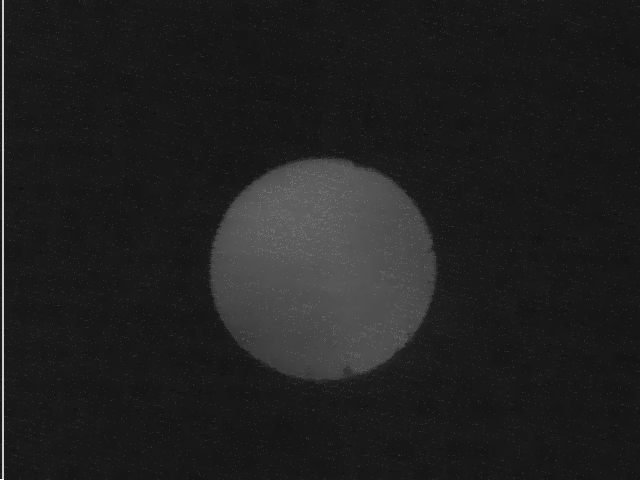
\includegraphics[width=\linewidth]{threshold-origin.png}
        \subcaption{测试原图像}\label{fig:thres-origin}
    \end{minipage} \hfill
    \begin{minipage}{0.48\linewidth}
        \centering
        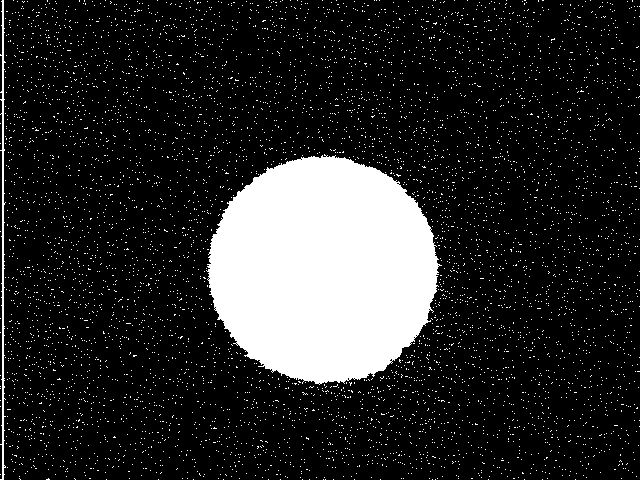
\includegraphics[width=\linewidth]{graymean.png}
        \subcaption{灰度平均值法}\label{fig:graymean}
    \end{minipage} \\
    \begin{minipage}{0.48\linewidth}
        \centering
        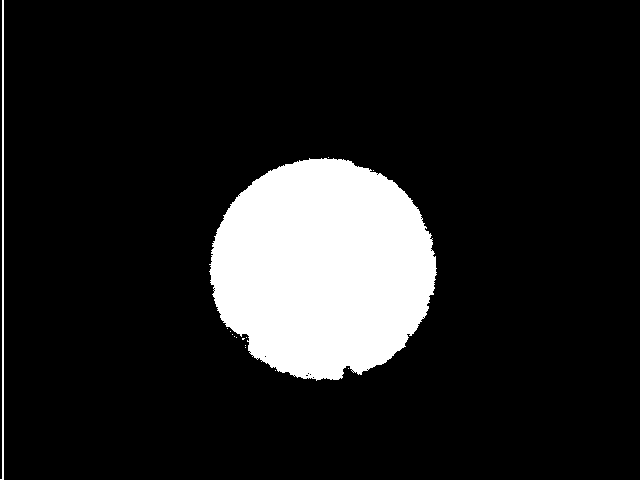
\includegraphics[width=\linewidth]{ptile.png}
        \subcaption{P-Tile比例阈值法($P=87\%$)}\label{fig:ptile}
    \end{minipage} \hfill
    \begin{minipage}{0.48\linewidth}
        \centering
        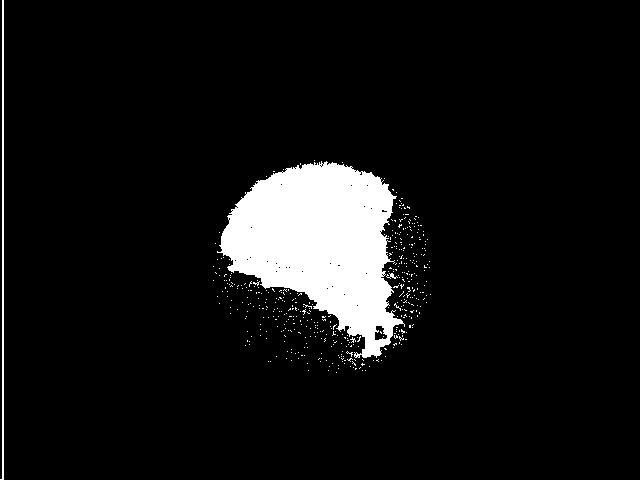
\includegraphics[width=\linewidth]{moment.png}
        \subcaption{力矩保持法}\label{fig:moment}
    \end{minipage} \\
    \begin{minipage}{0.48\linewidth}
        \centering
        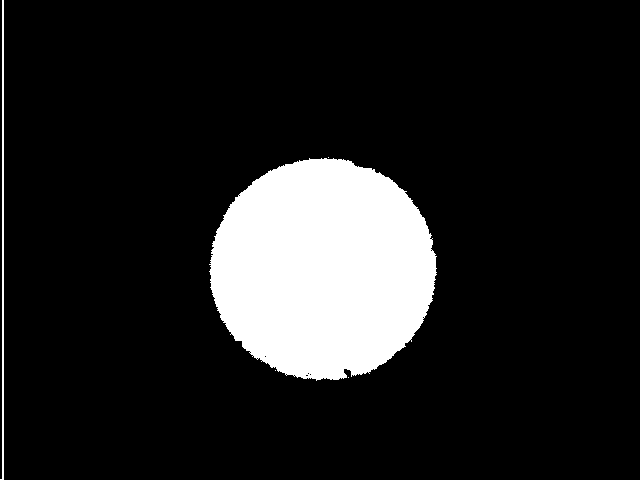
\includegraphics[width=\linewidth]{otsu.png}
        \subcaption{大津法}\label{fig:otsu}
    \end{minipage} \hfill
    \begin{minipage}{0.48\linewidth}
        \centering
        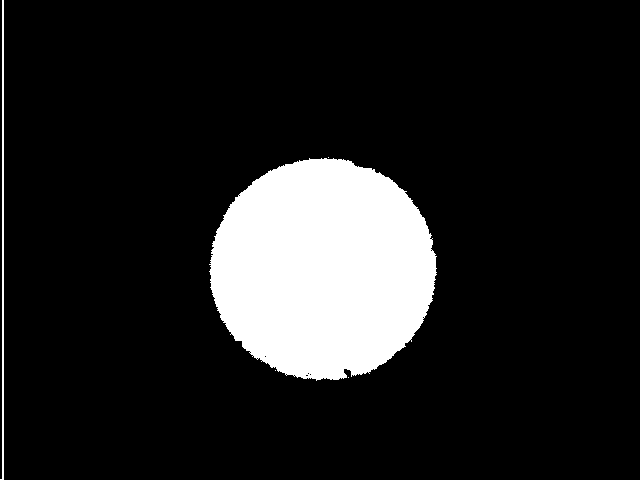
\includegraphics[width=\linewidth]{fuzziness.png}
        \subcaption{模糊度阈值分割法}\label{fig:fuzziness}
    \end{minipage}
    \caption{阈值分割算法测试}\label{fig:threshold}
\end{figure}

对经过均值平移滤波的B组图像进行二值化测试,结果如图\ref{fig:threshold}所示。
可以看到,灰度平均值法得到的阈值偏低,在二值图像中引入了大量噪声;
而力矩保持法得到的阈值偏高,导致二值图像中的目标图形显示不全。
P-Tile比例阈值法是半自动的阈值分割方法,选取合适的背景比例可以得到较好的二值图像,
但如果比值划分不够细致,同样也不能保证获得非常准确的图像形态(如图\ref{fig:ptile})。
而对于测试图像,大津法和模糊度阈值分割法得到的结果完全一致,也是效果最好的,
因此程序中推荐方案使用的是这两种方法。

\subsection{边缘检测算法}

在传统的Canny边缘算法\cite{Canny1986A}中,边缘检测算子是先于二值化进行的。
但在本方案中,边缘检测是后于二值化进行的。因而几种边缘检测算子的实际效果相差无几。

边缘检测算子是基于卷积的线性滤波,程序中用到的几种算子如表\ref{tab:edgeop}所示。

\renewcommand\arraystretch{1.2}
\begin{table}[!htb]
    \centering
    \caption{边缘检测算子}\label{tab:edgeop}
    \begin{tabular}{|c|c|}
        \hline
        算子 & 卷积核 \\
        \hline
        Sobel算子 & $
            \begin{pmatrix}
                -1 & 0 & 1 \\
                -2 & 0 & 2 \\
                -1 & 0 & 1
            \end{pmatrix}
            ,\ 
            \begin{pmatrix}
                \ 1 & \ 2 & \ 1 \\
                \ 0 & \ 0 & \ 0 \\
                 -1 &  -2 &  -1
            \end{pmatrix}
        $ \\
        \hline
        Prewitt算子 & $
            \begin{pmatrix}
                -1 & 0 & 1 \\
                -1 & 0 & 1 \\
                -1 & 0 & 1
            \end{pmatrix}
            ,\ 
            \begin{pmatrix}
                \ 1 & \ 1 & \ 1 \\
                \ 0 & \ 0 & \ 0 \\
                 -1 &  -1 &  -1
            \end{pmatrix}
        $ \\
        \hline
        Scharr算子 & $
            \begin{pmatrix}
                \ 3 & 0 & \ -3 \\
                 10 & 0 &  -10 \\
                \ 3 & 0 & \ -3
            \end{pmatrix}
            ,\ 
            \begin{pmatrix}
                \ 3 &  \ 10 & \ 3 \\
                \ 0 & \ \ 0 & \ 0 \\
                 -3 &   -10 &  -3
            \end{pmatrix}
        $ \\
        \hline
        Laplacian算子 & $
            \begin{pmatrix}
                0 & \ 1 & 0 \\
                1 &  -4 & 1 \\
                0 & \ 1 & 0
            \end{pmatrix}
        $ \\
        \hline
    \end{tabular}
\end{table}
\renewcommand\arraystretch{1}

几种方法中,Laplacian算子效果最好(边缘最细),
因而在程序中推荐的方案配置都使用的是Laplacian算子。

\subsection{圆拟合算法}

程序里提供了3种圆拟合算法:
\begin{description}
    \item[幼稚的拟合法] :\\
        通过平均值计算拟合,仅当数据点在圆上均匀分布时大致有效,参考意义不大。
    \item[简单代数拟合法] :\\
        通过使指标函数
        \begin{equation}
            f = \sum_i \left((x_i - x_c)^2 + (y_i - y_c)^2 - R^2\right)^2
        \end{equation}
        最小,对数据进行拟合。\\
        相比标准的最小二乘拟合的残差平方和最小化
        \begin{equation}
        \begin{split}
            g &= \sum_i \nu _i^2 \\
              &= \sum_i \left(\sqrt{(x_i - x_c)^2 + (y_i - y_c)^2} - R\right)^2
        \end{split}
        \end{equation}
        此方法存在一定的系统偏差\cite{Al2009Error}。
        \begin{equation}\label{eq:error}
        \begin{split}
            f &= \sum_i \left((x_i - x_c)^2 + (y_i - y_c)^2 - R^2\right)^2 \\
              &= \sum_i \left(\nu _i (\nu _i+2R) \right)^2 \\
              &\approx 4 R^2 \sum_i \nu _i ^2
        \end{split}
        \end{equation}
        如式\eqref{eq:error}所示,
        此方法可能会倾向于使$R$减小而不是单单使残差平方和最小来最小化指标函数,从而导致系统偏差。
        但此方法思路简单,实现容易,处理速度快,而且实测误差基本在半个像素以内,因此仍然使用此方法。
    \item[\ruby{超级}{Hyper}代数拟合法] \cite{Al2009Error}:\\
        结合了Pratt拟合法\cite{MR987653}和Taubin拟合法\cite{Taubin1991Estimation},
        拟合具有无偏性,但处理速度比前面的简单代数拟合法要稍慢。
\end{description}

\subsection{误差校正算法}

误差校正,准确地说是粗大误差的剔除,在原本的方案中并不存在。
但伴随着程序的调试,发现图像左侧边缘的白线对拟合处理的影响极大,
而且常规的滤波操作无法将其滤除,故考虑在拟合过程中加入校正环节。

最终在程序中使用了两种校正方法:
\begin{description}
    \item[中位误差校正] :\\
        迭代式算法。在得到初步拟合结果的条件下剔除误差大于误差中位数的点,
        按剩下的点重新拟合,如此往复,直到整体误差小于给定值为止。
        此方法受初始情况影响大,如果最初的拟合曲线就穿过了大量干扰点,
        则很可能无法收敛。
    \item[基于连通性的误差校正] :\\
        考虑到边缘算子得到的边缘图形必定是连通的,而干扰点与目标图形通常不会连通,
        故利用连通性作为判据可以分离干扰点和目标图形。
        再选取合适的判据分析所有连通区域中哪个最可能是目标图形,
        并以此区域进行拟合即得到结果。
        当干扰点较多时,此方法处理速度相对较慢,但准确性较好。
\end{description}

\section{实验结果}

如表\ref{tab:config}所示,程序附带的推荐方案有三份,分别用于A、B、C三组。

\begin{table}[!htb]
    \centering
    \caption{推荐方案配置}\label{tab:config}
    \begin{tabularx}{\textwidth}{|c|X|X|X|X|X|}
        \hline
        方案 & 滤波算法 & 阈值分割 & 边缘检测 & 圆拟合 & 误差校正 \\
        \hline
        a & 中值滤波 \newline 滤波半径:2 & 模糊度阈值分割 & Laplacian算子 & 简单代数拟合法 & 中位误差校正 \\
        \hline
        b & 均值平移滤波 \newline 空间滤波半径:1 \newline 色彩滤波半径:0.02 \newline 最大等级:20 & 大津法 & Laplacian算子 & 简单代数拟合法 & 基于连通性的误差矫正 \\
        \hline
        c & 高斯滤波 \newline 滤波半径:2 \newline 标准差:1.5 & 模糊度阈值分割 & Laplacian算子 & 超级代数拟合法 & 基于连通性的误差校正 \\
        \hline
    \end{tabularx}
\end{table}

\newcommand{\resultfig}[2]{
\begin{figure}[!htbp]
    \centering
    \subcaptionbox{边缘图像}{\includegraphics[width=0.48\linewidth]{#1#2-edge.png}}\hfill
    \subcaptionbox{拟合结果}{\includegraphics[width=0.48\linewidth]{#1#2-out.png}}
    \caption{#1组-方案#2}\label{fig:#1#2}
\end{figure}
}

\resultfig{A}{a}

\resultfig{A}{b}

\resultfig{A}{c}

\resultfig{B}{a}

\resultfig{B}{b}

\resultfig{B}{c}

\resultfig{C}{a}

\resultfig{C}{b}

\resultfig{C}{c}

各方案对各组图像的处理结果如图\ref{fig:Aa}\~{}\ref{fig:Cc}所示。
可以看到,方案a和方案c对各组图像都有效,而方案b对C组图像无法有效处理(图\ref{fig:Cb})。

\section{程序说明}

程序源码较长,就不附在报告里了。
完整源码可以在GitHub仓库
\url{https://github.com/miRoox/MEMS-oriented-image-testing-technology}
下的子目录
\href{https://github.com/miRoox/MEMS-oriented-image-testing-technology/tree/master/cpp-qt}{cpp-qt}
找到。

程序基于\href{https://www.qt.io/}{Qt}开发。
结构上,采用视图与模型分离的模式,使程序结构清晰,开发与调试便利;
行为上,操作和响应是异步进行的,将耗时的图像处理过程放置于单独的线程中,以避免界面操作被阻塞。

\newcommand{\reporef}[1]{\href{https://github.com/miRoox/MEMS-oriented-image-testing-technology/blob/master/cpp-qt/#1}{#1}}

源文件介绍:
\begin{itemize}
    \item \reporef{mems.pro} - qmake项目文件,提供项目管理和自动构建。
    \item \reporef{main.cpp} - 主函数所在文件,程序入口。
    \item \reporef{mainpanel.h}, \reporef{mainpanel.cpp} - 主面板,界面响应与控制。
    \item \reporef{mainpanel.ui} - 基于 Qt Designer 设计的主面板界面,构建时自动生成 ui\_mainpanel.h 。
    \item \reporef{processor.h}, \reporef{processor.cpp} - 处理器,负责处理图像。
    \item \reporef{algorithms.h} - 算法包装,包含了所用到的全部图像处理算法。
    \item \reporef{imagefilter.h}, \reporef{imagefilter.cpp} - 图像滤波与卷积算法。
    \item \reporef{binarize.hpp} - 二值化算法,header only。
    \item \reporef{thresholding.h}, \reporef{thresholding.cpp} - 阈值分割算法。
    \item \reporef{edgedetect.h}, \reporef{edgedetect.cpp} - 边缘检测算法。
    \item \reporef{circlefit.h}, \reporef{circlefit.cpp} - 圆拟合与误差矫正算法。
    \item \reporef{configuration.h}, \reporef{configuration.cpp} - 参数配置类,参数配置的包装。
    \item \reporef{thumbnailview.h}, \reporef{thumbnailview.cpp} - 缩略图预览控件。
    \item \reporef{progressupdater.h}, \reporef{progressupdater.cpp} - 进度条控制辅助类。
    \item \reporef{utils.h} - 杂项工具。
    \item \reporef{images.qrc} - Qt 资源文件,图像资源。
    \item \reporef{mems\_zh\_CN.ts} - Qt 翻译文件,中文翻译。
    \item \reporef{config.ini} - 配置文件,提供算法的默认配置。
\end{itemize}

\printbibliography[heading=bibliography,title=参考文献]

\end{document}
